
\chapter*{\label{ref-014}Leeuwarden en achterkleinkinderen}

\begin{figure}[h]
    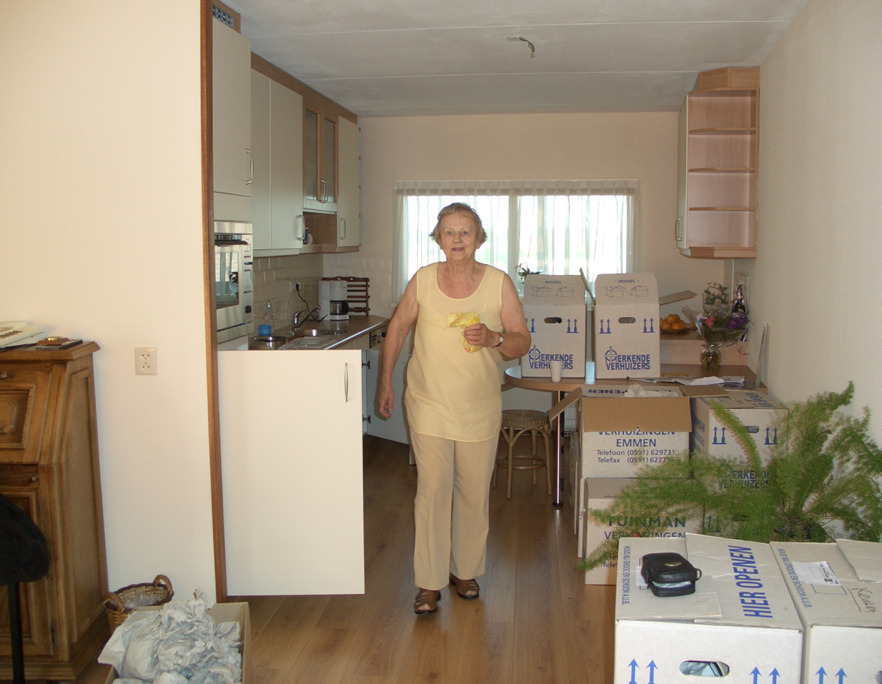
\includegraphics[width=\textwidth]{image68}
    \caption{In mijn nieuwe appartement in Leeuwarden.}
\end{figure}

\lettrine[lines=2, loversize=0.3, lraise=0]{\initfamily I}{n} 2007 heb ik het huis in Valthe verkocht want het werd me te veel. Ik was toen 79. Ik ben naar Leeuwarden verhuisd.

Ik vond dat best wel leuk, het was een nieuwe omgeving. Ook Lammie, mijn buurvrouw uit Valthe die naar Utrecht was verhuisd, vond zo’n nieuwe omgeving leuk. Ik ben een stuk gaan fietsen om alles te verkennen! Valthe was wel een paradijsje maar ik redde het onderhoud niet meer. Ik ben natuurlijk verschillende keren verhuisd en ik kon me overal wel weer settelen. 

En het was leuk om in de buurt van de kinderen te gaan wonen. 

\begin{figure}[h]
    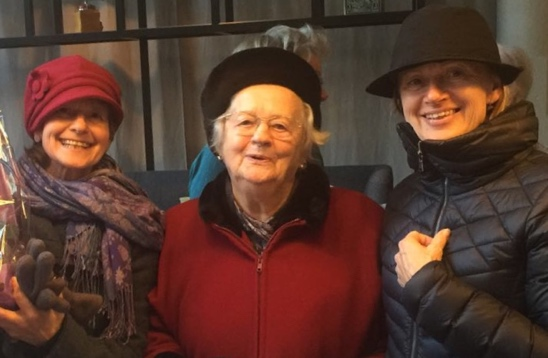
\includegraphics[width=\textwidth]{image69}
    \caption{Yvonne, ik, en Jacqueline.}
\end{figure}
\begin{figure}[h]
    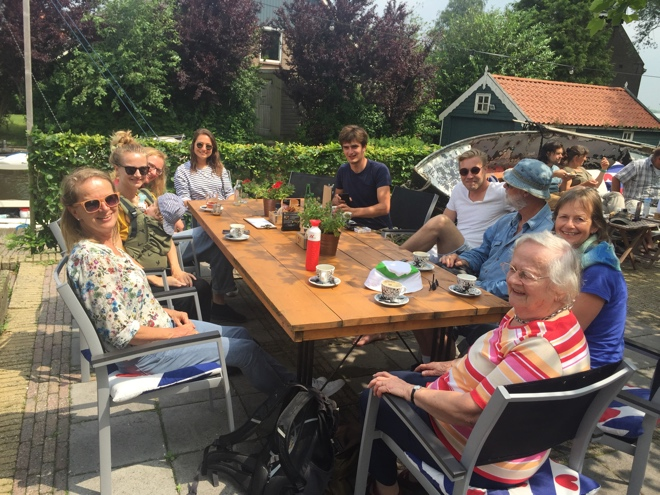
\includegraphics[width=\textwidth]{image70}
    \caption{Hier waren we met z'n allen een dagje varen.}
\end{figure}

Mensen zijn aardig hier, en ik heb hier een leuk plekje tussen de mannen in. De ene helft zit wel steeds in Zwiggelte in hun tweede huis (gelijk hebben ze) maar Niek komt elke vrijdag de klok bij me opwinden. Hij met zijn hond. De hond gaat dan gelijk voor het kastje liggen waar ik de hondenkoekjes bewaar! Ik heb ook een vriendin hier in het gebouw, Cobie. 

Ik vind het ook een fijn plekje, zo aan de buitenkant van de stad, en vlak bij het station, en het appartement is vrij ruim. Dat had ik altijd al bedacht dat je als je oud bent ruimte moet hebben in huis zodat je nog kunt lopen. Met het ouder worden gaat alles wel veel langzamer. 



Ik heb sinds ik hier woon vier achterkleinkinderen gekregen. Dat overkomt je maar gewoon! Het is enig om ze af en toe te zien.

Lisa komt soms met de trein met Eli. 

Celine’s kinderen zie ik ook wel als ze hier in Friesland zijn. 

Ik heb er ook nog een extra kleinzoon bij gekregen. Dorus, de pleegzoon van Jacqueline, hoort er wel echt bij voor mij.

Het leven is nu soms wel een beetje saai. Dan denk ik morgen ga ik eens wat doen en dan is die morgen zomaar weer voorbij! Ik ben wel blij dat ik hier woon met de kinderen vlakbij. Ik loop nog en ik kan nog dingen; ik ga me geen zorgen maken over hoe het verder gaat. En Fokje helpt me. 

Laatst (zomer 2020) heeft Yvonne me een dag meegenomen naar zee, bij Camperduin en Schoorl. Dat was wel erg leuk! Ik was toen 92. Nou, zo vind ik het wel genoeg!

\begin{figure}[h]
    \begin{centering}
    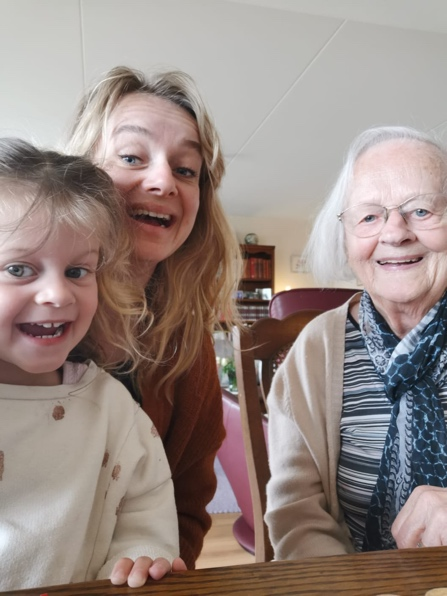
\includegraphics[width=\textwidth]{image72}
    \caption{Mijn achterkleindochter Eli en mijn kleindochter Lisa.}
    \end{centering}
\end{figure}

\begin{figure}[h]
    \begin{centering}
    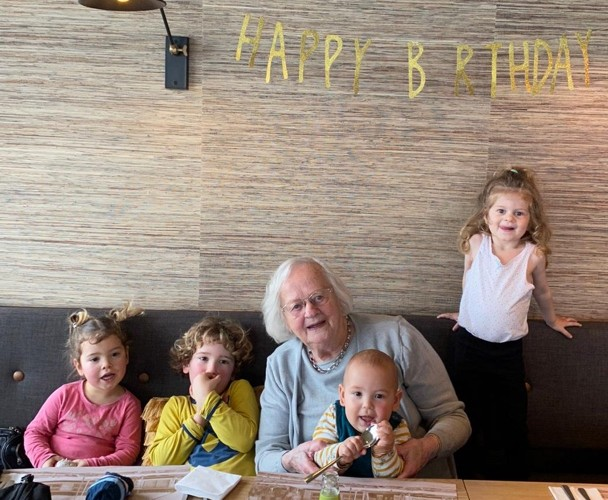
\includegraphics[width=\textwidth]{image71}
    \caption{Met de achterkleinkinderen.}
    \end{centering}
\end{figure}

\newpage
\thispagestyle{empty}
\pagestyle{empty}

\begin{figure}[h]
    \begin{centering}
    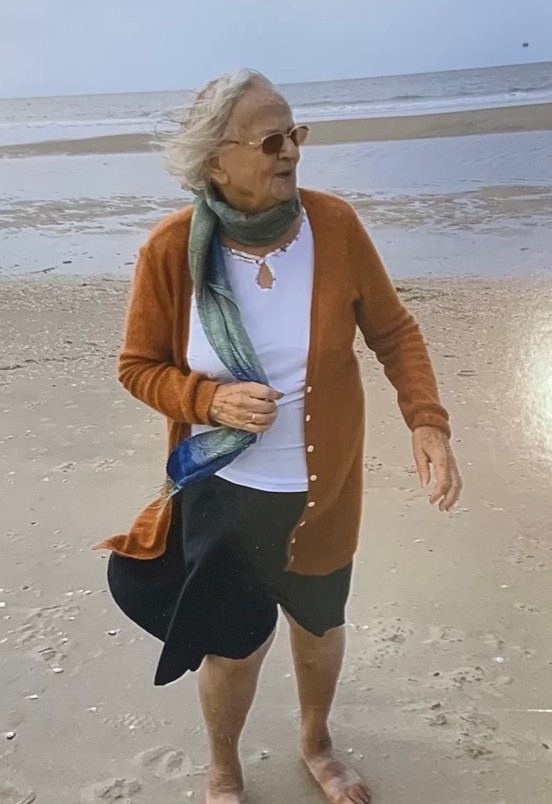
\includegraphics[width=\textwidth]{image73}
    \caption{Bij Camperduin en Schoorl op het strand, 92 jaren jong.}
    \end{centering}
\end{figure}